%==============  code_only_box.tex  =================
\documentclass[11pt]{article}

% 레이아웃/폰트 (필요 없으면 빼도 됨)
\usepackage{geometry}
\geometry{margin=1in}
\usepackage{fontspec}
\usepackage[space]{xeCJK}          % ← minted와의 verbatim 충돌 피하려면 [space] 옵션은 쓰지 마세요
\setCJKmainfont{Noto Sans KR}

\usepackage{setspace}
\setstretch{1.2}
\setlength{\parindent}{0pt}
\setlength{\parskip}{6pt}


% tcolorbox + (minted|listings) 토글
\newif\ifuseminted
\usemintedtrue             % minted 사용(하이라이트 예쁨). 안 되면 false로 바꿔 listings 사용

\usepackage[many]{tcolorbox}
\tcbuselibrary{skins,breakable,listings,minted}
\usepackage{xcolor}
\definecolor{codebg}{RGB}{248,248,248}
\usepackage{enumitem}          % ★ 필요
\usepackage{graphicx}
\usepackage{float}
% --- minted 버전: "코드 전용" 박스 (listing only)
\ifuseminted
  \usepackage{minted}       % 컴파일: xelatex -shell-escape code_only_box.tex
  \newtcblisting{CodeBox}[1][]{
    enhanced, breakable,
    colback=codebg, frame hidden,
    boxrule=0pt, borderline={0.5pt}{0pt}{black!15, dashed},
    sharp corners, before skip=8pt, after skip=12pt,
    listing engine=minted,
    listing only,            % ★ 박스 안엔 오직 코드만
    minted language=python,  % 필요 시 \begin{CodeBox}[minted language=c++] 로 덮어쓰기
    minted options={
      fontsize=\small,
      breaklines,
      autogobble,
      linenos,
      numbersep=6pt,
      tabsize=2
    },
    #1                       % 사용자 옵션 전달
  }
\else
% --- listings 버전: shell-escape 불가 시
  \usepackage{listings}
  \lstdefinestyle{mylist}{
    basicstyle=\ttfamily\small,
    numbers=left, numbersep=6pt,
    breaklines=true,
    tabsize=2,
    backgroundcolor=\color{codebg},
    showstringspaces=false
  }
  \newtcblisting{CodeBox}[1][]{
    enhanced, breakable,
    colback=codebg, frame hidden,
    boxrule=0pt, borderline={0.5pt}{0pt}{black!15, dashed},
    sharp corners, before skip=8pt, after skip=12pt,
    listing engine=listings,
    listing only,            % ★ 박스 안엔 오직 코드만
    listing options={style=mylist, language=Python},
    #1
  }
\fi



\begin{document}

\begin{center}
  {\LARGE \bfseries Graph based Block Digonalization 코드 주석 정리} \\[10pt]
  {\large 최윤호}
\end{center}

\section{분자(화합물) 정의}
\begin{CodeBox}[title={Example: Python snippet}]
geometry = [('H', (0., 0., 0.)),
            ('H', (dist, 0., 0. )),
            ('H', (2*dist, 0., 0. )),
            ('H', (3*dist, 0., 0.))]  # Angstrom
basis = 'sto-3g'
mol = MolecularData(geometry, basis, multiplicity=1, charge=0)
# qiskit 의 molecularinfo 와 같이 분자의 정보를 담고있는 클래스를 생성 이때 필요한 정보는 기하학적인 구조(geometry), basis, 시스템의 multiplicity와 총 전하량 등의 정보가 필요하다. 
\end{CodeBox}

\begin{enumerate}[label=\textbf{*}, leftmargin=*]
  \item geometry : 원자의 종류와 기하학적인 구조를 튜플로써 저장 ('원소종류', (x,y,z))
  \item basis : 전자의 atomic orbital 을 표현할 basis 설정 (sto3g, 6-31g,$\cdots$)
  \item MolecularData: qiskit 의 molecularinfo 와 같이 분자의 정보를 담고있는 클래스
\end{enumerate}
이는 객체는 분자(화합물)의 정보를 담고있는 객체로써, 이후 이 객체로부터 전자의 개수나, scf 계산을 수행할것이다. 
이번 논문에서 사용한 화합물은 H2 Cluster 로써 아래와같이 모든 수소원자가 같은 거리만큼 떨어져있는 구조를 의미한다. 
\begin{figure}[h]
    \centering
    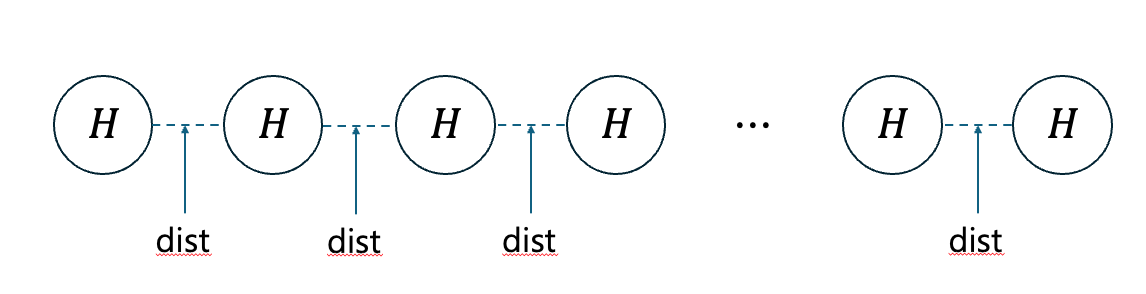
\includegraphics[width=0.8\textwidth]{/Users/choeyunho/Documents/mygit/2025_GBBD/코드_주석/fig/h2cluster.png}
    \caption{H2 Cluster}
    \label{fig:my_image}
\end{figure}


\section{FCI 행렬 생성}
\begin{CodeBox}[title={Example: Python snippet}]
mol = run_pyscf(mol_input, run_scf=1, run_fci=0)
# mol_input : 앞서 MolecularData 클래스를 이용해 생성된 객체 분자의 여러 정보를 담고있다. 
# run_pyscf : mol_input 을 바탕으로 계산을 수행 2nd Quantized 헤밀토니안을 얻기위한 HF 계산을 수행한다. 
# 이때 옵션으로 여기서 FCI 계산을 수행할수도 있으나, 이는 Cost가 매우커서 수행하지 않는다. 
ham_int = mol.get_molecular_hamiltonian()
# pyscf 계산을 수행한 이후 정보를 담고있는 mol 이라는 객체로 부터 1차/2차 적분에 대한 정보를 가져온다. 
# (*) 이후 객체 정보에 대한 추가설명
ham_fci = get_fermion_operator(ham_int)
# 1차/2차 적분에 대한 정보를 담고있는 ham_int로 부터 2nd Quantized된 헤밀토니안을 가져온다. 
# (**) 이후 객체 정보에 대한 추가설명 

H = get_number_preserving_sparse_operator(
# 전자수 와 스핀량 보존을 포함하는 FCI 행렬을 만들기 위한 함수
fermion_op=ham_fci, #사용할 2nd Quantized 헤밀토니안
num_qubits=mol.n_qubits, #총 스핀오비탈 개수 openFermion 패키지에서는 이를 qubit 라는 이름으로 사용하지만, 같은 의미.
num_electrons=mol.n_electrons,  # 시스템의 전자수 
spin_preserving=True)        # 시스템의 multiplicity가 보존되는 Determinant 만을 사용
H_real = H.real # 행렬의 각 원소는 두 Determinant로 기술되는 내적이며 이는 에너지에 대응되는 값이므로 실수값을 갖게되므로, 이후 그래프 연산을 위해 실수로 변환
# (***) 이후 객체 정보에 대한 추가설명 
\end{CodeBox}
\newpage
\subsection{(*) mol.get\_molecular\_hamiltonian()}
1차, 2차 적분의 결과를 아래와같이 저장 한다. 
\begin{figure}[H]
    \centering
    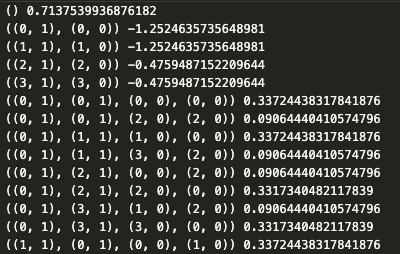
\includegraphics[width=0.3\textwidth]{/Users/choeyunho/Documents/mygit/2025_GBBD/코드_주석/fig/ham_int.png}
    \caption{molecular Hamiltonian}
    \label{fig:my_image}
\end{figure}
\begin{enumerate}[label=\textbf{*}, leftmargin=*]
  \item () : 가장 위의 공란은 Constant 값 (여기서는 핵간 척력) 
  \item ((0,1),(0,0)) : 튜플의 튜플로 정의 된다. 안의 튜플은 순서대로 (연산이 수행되는 오비탈 idx, 생성(1)인지, 소멸(0)인지) 결국 second Quantization 에서 1차여기항에 대응된다. 
  \item ((0, 1), (0, 1), (0, 0), (0, 0)) : 튜플 4개로 정의 된다. 안의 튜플은 위에서와 같은 정보를 사용. 결국 second Quantization 에서 2차여기항에 대응된다. 
\end{enumerate}

\subsection{(**) get\_fermion\_operator(ham\_int)}
1차, 2차 적분의 결과를 아래와같이 fermionic 생성/소멸 연산자의 표기법을 통해 2nd Quantized 해밀토니안으로 표현한다. 
\begin{figure}[H]
    \centering
    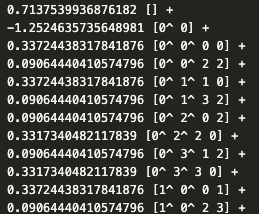
\includegraphics[width=0.3\textwidth]{/Users/choeyunho/Documents/mygit/2025_GBBD/코드_주석/fig/ham_fci.png}
    \caption{fermionic op}
    \label{fig:my_image}
\end{figure}
여기서, 
\begin{center}
[] : Constant 값 (여기서는 핵간 척력) 

[i\textasciicircum  j] : $a^{\dagger}_i a_j $ 

[i\textasciicircum  j\textasciicircum k l] : $a^{\dagger}_i a^{\dagger}_j a_k a_l $ 
\end{center}

\newpage

\subsection{(***) get\_number\_preserving\_sparse\_operator()}
아래와같이 희소행렬 표현으로 FCI 행렬을 구성한다. 
\begin{figure}[H]
    \centering
    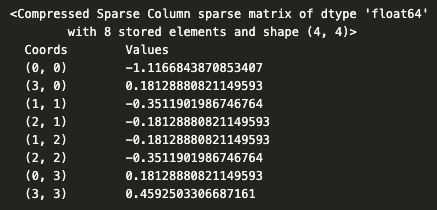
\includegraphics[width=0.8\textwidth]{/Users/choeyunho/Documents/mygit/2025_GBBD/코드_주석/fig/h_matrix.png}
    \caption{FCI matrix}
    \label{fig:my_image}
\end{figure}

\newpage

\section{FCI 행렬 -> 그래프로 변경}

\begin{CodeBox}[title={Example: Python snippet}]
def sparse_to_graph(A):
    """
    희소행렬 A -> NetworkX Graph/DiGraph 변환

    Returns
    -------
    G : nx.Graph
    """
    
    if not issparse(A):
        raise ValueError("A must be a scipy.sparse matrix")
    
    # COO로 변환
    A = A.tocoo(copy=True)
    #COO 에서는 값을 아래와같이 3개의 어레이로 저장 
    #data : [3,4,2,7]
    #row : [0,0,1,3]
    #col : [2,4,1,3]
    #그리고 같은 인덱스 순서대로 0행 2열에는 3이라는 값이 있고 마찬가지로 총 4개의 원소가 있는 행렬을 표현한다. 

    G = nx.Graph()
    # NetworkX 패키지의 Graph 클래스를 불러온다. 
    G.add_nodes_from(range(A.shape[0]))  # 노드: 0..n-1
    # A(coo matrix) 의 길이, 즉 행렬의 원소의 개수만큼의 node를 만든다. 
    vals = np.abs(A.data)
    # 행렬의 데이터 (이경우 h_ij) 를 하나의 어레이로 만든다. 

    # 동일 엣지 중복 합치기(무향일 때 i<j 묶기)
    from collections import defaultdict
    edges = defaultdict(float)
    # 딕셔너리를 만들때, 특정 키가 주어졌을때, 그 키가 만약 존재하지 않다면 0.0 이라는 값을 그 키로 하는 value 를 만든다. 
    for i, j, v in zip(A.row, A.col, vals):
    # 행(i), 열(j), 행렬원소(h_ij)
        if i == j :
            continue
            # 대각원소는 자기와의 간선이므로, 이는 고려하지 않는다. 
        key = (min(i, j), max(i, j))
        # key를 만들어 이를 이용해 간선(edges) 를 만들것이다. 
        # 그런데, ''무향'' 그래프 에선 두 노드 사이의 방향이 없으므로
        # h_ij 와 h_ji 를 같은 키로 만들어 위와같이 정의한다. 
        edges[key] += 0.5*float(v) 
        # 누적(합)
        # key를 정의할때 (min(i, j), max(i, j))와 같이 했으므로 
        # h_ij 와 h_ji 는 같은 key에 대응되고, 이 두 값은 하나의 edge 에 대응되어야한다. 
        # 우리가 다루는 행렬에서는 이 두 값이 같으므로, 두값을 평균을 내어 처리한다. 

        for (i, j), w in edges.items():
        # 저장된 딕셔너리에서 키인 (i,j) 와 그때의 행렬원소 (h_ij)를 for문으로 가져온다.
            G.add_edge(i, j, weight=w)
            # 그래프에 i번째 노드와 j번째 노드의 간선으로써 행렬원소 (h_ij)를 부여한다. 

    return G # NetworkX 패키지의 Graph 클래스에 노드와 간선들이 저장되어있는 객체
\end{CodeBox}

\subsection{sparse 행렬표현 VS COO 행렬표현}
아래와같은 행렬이 있다고 해보자.
\[
A = \begin{bmatrix}
5 & 0 & 0 & 1 \\
0 & 2 & 0 & 0 \\
3 & 0 & 0 & 4 \\
0 & 0 & 6 & 0
\end{bmatrix}
\]

\subsubsection*{어레이로 표현}
가장 파이썬에서 이러한 행렬을 일반적으로 아래와같이 저장한다. 
\begin{CodeBox}[title={Example: Python snippet}]
A = [[5, 0, 0, 1],[0, 2, 0, 0],[3, 0, 0, 4],[0, 0, 6, 0]]
\end{CodeBox}
하지만 우리가 다루는 행렬은 매우 큰 행렬이고, 우리의 FCI 행렬은 0인성분이 많기때문에 위와같이 저장하는것은 비효율적이다. 
그래서 다음의 방식을 사용한다. 

\subsubsection*{희소행렬표현}
0이 아닌성분이 우리가 다뤄야할 주된 값이고, 이 값이 전체 행렬에서 희소하기 때문에 위 행렬을 아래와같이 저장할 수 있다. 
\begin{CodeBox}[title={Example: Python snippet}]
Coords  Values
(0, 0)  5
(0, 2)  3
(1, 1)  2
(2, 3)  6
(3, 0)  1
(3, 2)  4
\end{CodeBox}

0이 아닌 값들과 그 좌표를 통해 데이터를 저장한다. 

\subsubsection*{Coo 행렬표현}
비슷한 형태로써 아래와같이 저장을할 수 있다. NetworkX 패키지에서 행렬을 취급할때 이 방식과 같이 저장하게된다. 
\begin{CodeBox}[title={Example: Python snippet}]
data = [5, 1, 2, 3, 4, 6]
row  = [0, 0, 1, 2, 2, 3]
col  = [0, 3, 1, 0, 3, 2]
A_coo = coo_matrix((data, (row, col)), shape=(4, 4))
\end{CodeBox}
0이 아닌 값들의 리스트와 각 값의 행, 열에 대한 리스트를 만든다.
데이터 리스트에서 i번째 값이 열 리스트에서 i번재 열, 행 리스트의 i번째 행에 있는 행렬을 나타낸다. 

\section{main 에너지 계산 함수}
위의 두 내용을 이용하여 에너지 계산에 사용
% 박스 안: 원문 코드만
\begin{CodeBox}[title={Example: Python snippet}]
def GBBD(mol):
  # 입력 : qiskit 의 molecule info 와 같이 분자의 정보를 담고있는 클래스인 MolecularData
  # 이후에 추가 설명
  mol = run_pyscf(mol, run_scf=1, run_fci=0)
  # 3. 2차 정량화 Hamiltonian 얻기
  ham_int = mol.get_molecular_hamiltonian()
  ham_fci = get_fermion_operator(ham_int)     
  #H = get_sparse_operator(ham_fci, n_qubits=mol.n_qubits)
  H = get_number_preserving_sparse_operator(
  fermion_op=ham_fci,
  num_qubits=mol.n_qubits,
  num_electrons=mol.n_electrons,       # 필수
  spin_preserving=True ,        # S_z 고정 (필요 없으면 None)
  reference_determinant=None,
  excitation_level=None)
  print(H)
  H_real = H.real
  '''
  --------------
  메인코드에서 이부분까지는 2(FCI 행렬 생성) 에서 설명
  H_real : i,j 번째 Slater Determinant 의 헤밀토니안 에대한 내적값으로 기술된 행렬 (=FCI 행렬)
  # 이를 대각화 하여 계산하는것이 FCI
  # sparse 행렬로 표현됨. 
  '''
  G = sparse_to_graph(H_real)
  # 3(FCI 행렬 -> 그래프로 변경) 에서 정의한 함수를 통해 H_real 행렬을 G 라는 그래프의 형태로 인코딩
  ccs = list(nx.connected_components(G))
  # nx.connected_components() 함수를 통해 G 라는 그래프 객체에서, 연결된 노드들을 묶어서 표현.
  # Closed loop 라기보다는, 각 노드들간 을 이동할 수 있다면 그는 하나의 연결요소로 택한다. 
  '''
  여기까지의 과정이 헤밀토니안 행렬을 그래프를 이용해서 Block 짓는 과정. 
  즉, 서로 연관성이 있는 basis(Slater Determinant) 끼리 묶어 부분 행렬을 생성
  ''' 

  sub_mat_idx_g = list(ccs[0])
  # nx.connected_components(G) 를 통해 생성된 묶음들 중에서 0번 idx, 
  # 즉 제일 큰 묶음을 나타내는 그래프의 인덱스를 저장
  H_sub_g = H[sub_mat_idx_g, :][:, sub_mat_idx_g]
  # 제일 큰 묶음에 포함되는 인덱스들만을 이용하여 부분행렬을 생성.
  print(H_sub_g)
  # 이를 확인용으로 출력 
  eigval_g, eigvec = eigsh(H_sub_g, k=1, which='SA')
  # 이 부분행렬을 대각화 
  E_g = eigval_g[0]
  # 제일 큰 묶음으로 구성된 부분행렬의 가장 작은 고윳값이 바닥상태 에너지에 대응된다. 
  # 이를 E_g 로 저장. 

  sub_mat_idx_e = list(ccs[1])
  # 즉 제일 "두번째로 큰" 묶음을 나타내는 그래프의 인덱스를 저장
  H_sub_e = H[sub_mat_idx_e, :][:, sub_mat_idx_e]
  # 마찬가지로 이를 이용해 부분행렬을 생성
  print(H_sub_e)
  # 확인용 출력
  eigval_e, eigvec = eigsh(H_sub_e, k=1, which='SA')
  # 이 부분행렬을 대각화 
  E_e = eigval_e[0]
  # 두번째로 큰 묶음으로 구성된 부분행렬의 가장 작은 고윳값이 1차 여기 상태 에너지에 대응된다. 
  # 이를 E_g 로 저장. 

  return E_g, E_e # 바닥상태 에너지와 1차 여기상태 에너지를 함수의 결과로 출력.
\end{CodeBox}

\section{예시코드 ($H_2$ PES)}
PES 란 Potential Energy Surface 로 분자의 거리를 변화시켜가며 에너지를 플롯한 그래프를 의미한다. 
논문에서 여러 H2 클러스터에 대해서 이 PES를 얻은 결과가 있는데, 이를 얻기위한 계산이다. 
\begin{CodeBox}[title={Example: Python snippet}]
#H2
H2_energy_arr_g = []
H2_energy_arr_e1 = []
# GBBD 함수에서는 바닥상태 에너지와 1차여기상태 에너지를 출력하므로, 
# 이 두가지를 담을 리스트를 준비한다. 
for dist in np.arange(0.4,2.5, 0.1):
# 단위는 Angstrom이며, 0.4 부터 2.5 까지 거리를 0.1 만큼 변화시켜가며 에너지를 계산한다. 
    geometry = [('H', (0., 0., 0.)),
                ('H', (dist, 0., 0.))]
    # 위 H2 Cluster 구조에서 알 수 있듯이 두 수소원자는 dist 만큼 떨어져있어야하므로
    # x축을 기준으로 dist 만큼 떨어져 있도록 기하학적 구조를 설정
    basis = 'sto-3g'
    # toy model 의 계산이므로 basis는 가장 작은 sto-3g를 사용 
    mol = MolecularData(geometry, basis, multiplicity=1, charge=0)
    # 기하학적 구조와 basis, 그리고 H2분자의 spin과 전하를 고려하여 파라미터를 주고 
    # MolecularData() 함수를 통해 mol 이라는 객체를 생성
    energy_g, energy_e1 = GBBD(mol)
    # 입력 : 분자의 기하학적인 구조를 담고있는 객체 (mol)
    # 출력 : 바닥상태 에너지, 1차 여기상태 에너지 
    H2_energy_arr_g.append(energy_g)
    H2_energy_arr_e1.append(energy_e1)
    # GBBD 함수의 두 결과를 각각 다른 리스트에 저장

\end{CodeBox}


\end{document}